% \documentclass[12pt]{article}

%%v helpful MIT exam schema, see http://www-math.mit.edu/~psh/exam/examdoc.pdf
 \documentclass[12pt]{exam} 
% \qformat{\textbf{Question \thequestion}\quad \thepoints\hfill } % Large depth to make space}
 \renewcommand{\thesubpart}{(\roman{subpart})}
 \renewcommand{\subpartlabel}{\thesubpart}
% \footer{}{}{Page \thepage\ de \numpages}
\addpoints
\pointsinmargin
% \boxedpoints
\renewcommand{\questionshook}{\setlength{\itemsep}{4mm}}
\renewcommand{\partshook}{
	\setlength{\itemsep}{0.2cm}
}

\usepackage{cmbright}

\pagestyle{empty} %for handouts
\addtolength{\jot}{2em} % this makes all formulae a bit more spaced vertically for handouts
\setlength{\parindent}{0pt} %we're not writing a novel
\renewcommand{\arraystretch}{1.5} %makes tables taller, so easier to write in

\usepackage[fleqn]{amsmath}
\usepackage{amssymb} %standard classy maths symbols
\usepackage[a4paper, margin=1in]{geometry} %makes it easy to specify where to put stuff on the page

\usepackage{siunitx} %v handy way of getting SI units to typeset correctly...
% \sisetup{locale = FR} %... and now it will use a comma for decimals

\usepackage[utf8]{inputenc}

% \usepackage[french]{babel} % frenchify everything (e.g. a Table becomes a Tableau)
% \usepackage{lmodern} % font with nicer French characters than standard
% \usepackage{textcomp} % and more help for special characters

\usepackage{tcolorbox} % basic but good package for boxes around text
\tcbset{colback=black!5!white}
% \usepackage{color} % colours
%\newcommand{\fillin}{\color{black!1!white}} %makes the text disappear
%\definecolor{fillin}{rgb} {1.00,1.00,1.00}
%\renewcommand{\fillin}{\color{blue}} \definecolor{fillin}{rgb} {0.00,0.00,1.00} %makes the filling in text appear (in blue)

\usepackage{enumitem} % can change the labels on lists, items, enumerates
\usepackage{setspace}

\usepackage{tikz, tkz-euclide} % interval diagrams, sets, etc.
%\usetikzlibrary{calc,trees,positioning,arrows,fit,shapes}

\begin{document}

\textbf{Name:} \dotfill

\
\begin{questions}


\question[2] Write down the equation for the area of a circle of radius $r$.
\fillwithdottedlines{7mm}
Determine the area of a sector of radius 10 and angle $30^\circ$.
\vspace{-5mm}

\begin{minipage}{0.8\textwidth}
\fillwithdottedlines{21mm}
\end{minipage}
\hspace{4mm}
\begin{minipage}{0.1\textwidth}
\vspace{5mm}

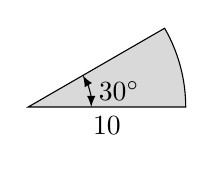
\begin{tikzpicture}
\draw[fill=black!15] (0,0) -- node[below] {10} (0:2) arc(0:30:2) -- cycle;
\draw[latex-latex]  (0:0.8) arc(0:30:0.8) node[midway, right]{$30^\circ$};
\end{tikzpicture}

\end{minipage}


\question[4] Find the shaded areas. \emph{State a formula before using it!}

\begin{minipage}{0.7\textwidth}
\fillwithdottedlines{70mm}
\end{minipage}
\begin{minipage}{0.3\textwidth}
\begin{center}

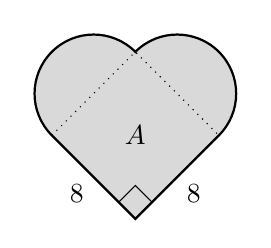
\begin{tikzpicture}[scale=1.5, rotate=45]
\draw[thick, fill=black!15] (0, 0)  -- (0,1) -- (0,1) arc(180:0:0.5cm) -- (1,1) arc(90:-90:0.5cm) -- cycle;
\draw[dotted] (0,1)--(1,1)--(1,0);
\draw (0,0) rectangle ++(0.2, 0.2);

\node at (0.5, -0.2) {8};
\node at (-0.2, 0.5) {8};
\node at (0.5, 0.5) {$A$};
\end{tikzpicture}


\vspace{3mm}

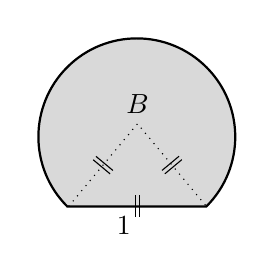
\begin{tikzpicture}[scale=2.5]
\coordinate (A) at (0,0);
\coordinate (B) at (0.7,0);
\coordinate (C) at (0.35,0.42);

\draw[thick, fill=black!15] (0, 0)  -- node[pos=0.4, below] {1} (0.7,0) -- (0.7,0) arc(-45:225:0.5cm) -- cycle;
\draw[dotted] (0,0)--(C) node[above] {$B$} --(0.7,0);
\tkzMarkSegment[pos=.5,mark=||](A,B) 
\tkzMarkSegment[pos=.5,mark=||](C,B) 
\tkzMarkSegment[pos=.5,mark=||](A,C) 


\end{tikzpicture}


\end{center}
\end{minipage}

\vfill

\question \textbf{Bonus.} 
Can you show that the two different shaded areas have the same area?
\vspace{-4mm}

\begin{center}
\def\leftcircle{(-2,0) circle (2cm)}
\def\upcircle{(0,2) circle (2cm)}
\def\bigcircle{(0,0) circle (4cm)}

\begin{tikzpicture}
\clip (-4.1,-0.01) rectangle (0.01,4.1);
    \fill[black!35] \bigcircle;
    \fill[white] \leftcircle;
    \fill[white] \upcircle;
    
    % Now we want to highlight the intersection of the first and the
    % second circle:

    \begin{scope}
      \clip \leftcircle;
      \fill[black!10] \upcircle;
    \end{scope}

    \draw[thick] (-4,0) -- (0,0) -- (0,4);
    \draw[thick] \leftcircle;
    \draw[thick] \upcircle;
    \draw[thick] \bigcircle;

\end{tikzpicture}
\end{center}


\end{questions}

\begin{tcolorbox}

\textbf{Name of the marker:}

\begin{center}
\gradetable[h][questions]
\end{center}

\end{tcolorbox}

\end{document}